\documentclass[12pt, a4paper]{article}
\usepackage[utf8]{inputenc}
\usepackage[T1]{fontenc}
\usepackage[french]{babel}
\usepackage{graphicx}
\usepackage{fancyhdr}
\usepackage{geometry}
\usepackage{listings}
\usepackage{xcolor}
\usepackage{float}
\usepackage{tcolorbox}
\usepackage{enumitem}

\usepackage[
    bookmarks=true,
    bookmarksopen=true,
    bookmarksnumbered=true,
    pdfusetitle,
    colorlinks=true,
    linkcolor=blue,
    urlcolor=blue,
    pdfborder={0 0 0}
]{hyperref}

\geometry{top=2.5cm, bottom=2.5cm, left=2.5cm, right=2.5cm}

% Configuration des listes
\setlist[itemize]{itemsep=0.5em, parsep=0.3em}
\setlist[enumerate]{itemsep=0.5em, parsep=0.3em}

% Définition des couleurs pour le code
\definecolor{codegreen}{rgb}{0,0.6,0}
\definecolor{codegray}{rgb}{0.5,0.5,0.5}
\definecolor{codepurple}{rgb}{0.58,0,0.12}
\definecolor{backcolour}{rgb}{0.95,0.95,0.92}

% Configuration du style de code
\lstdefinestyle{formulastyle}{
    backgroundcolor=\color{backcolour},   
    commentstyle=\color{codegreen},
    keywordstyle=\color{magenta},
    numberstyle=\tiny\color{codegray},
    stringstyle=\color{codepurple},
    basicstyle=\ttfamily\footnotesize,
    breakatwhitespace=false,         
    breaklines=true,                 
    captionpos=b,                    
    keepspaces=true,                 
    showspaces=false,                
    showstringspaces=false,
    showtabs=false,                  
    tabsize=2,
    frame=single,
    literate={é}{{\'e}}1 {è}{{\`e}}1 {à}{{\`a}}1 {ç}{{\c{c}}}1 {ù}{{\`u}}1 {ê}{{\^e}}1 {î}{{\^i}}1 {ô}{{\^o}}1 {û}{{\^u}}1 {ë}{{\¨e}}1 {ï}{{\¨i}}1 {ü}{{\¨u}}1 {Ç}{{\c{C}}}1
}

\lstset{style=formulastyle}

% Définition des styles de boîtes
\newtcolorbox{note}{
    colback=blue!5,
    colframe=blue!75!black,
    title=Note,
    fonttitle=\bfseries
}

\newtcolorbox{warning}{
    colback=red!5,
    colframe=red!75!black,
    title=Attention !,
    fonttitle=\bfseries
}

\newtcolorbox{tip}{
    colback=green!5,
    colframe=green!75!black,
    title=Astuce,
    fonttitle=\bfseries
}

\makeatletter
\def\maketitle{
    \begin{titlepage}
        \centering
        \vspace*{2cm}
        
        % Logo
        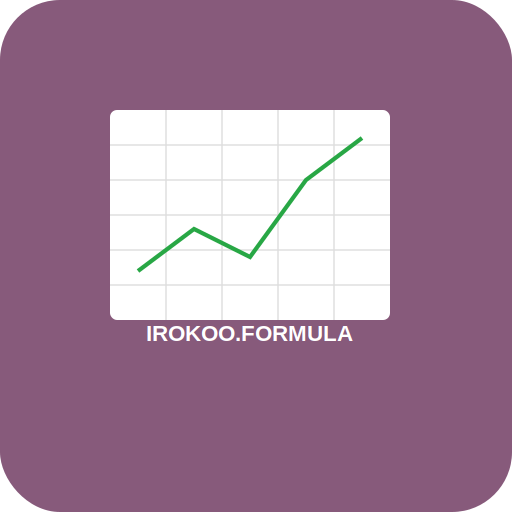
\includegraphics[width=0.4\textwidth]{../icon.png}
        \vspace{2cm}
        
        % Titre
        {\huge\bfseries Documentation Formules\\Spreadsheet Evolution\par}
        \vspace{2cm}
        
        % Auteur
        {\Large\itshape Sylvain Boutet\par}
        \vspace{1cm}
        
        % Date
        {\large \@date\par}
        
        \vfill
        
        % Pied de page
        {\large Odoo Version 18.0\par}
    \end{titlepage}
}
\makeatother

\title{Documentation des Formules Odoo Spreadsheet}
\author{IROKOO}
\date{\today}

% Début du document
\begin{document}

\maketitle
\tableofcontents
\newpage

\section{Introduction}

Le module \textbf{Spreadsheet Evolution} étend les fonctionnalités des feuilles de calcul Odoo en ajoutant des formules avancées permettant d'exploiter pleinement les données du système directement dans vos spreadsheets sans export préalable.

Ces formules permettent :
\begin{itemize}
    \item L'accès direct aux champs de n'importe quel enregistrement dans Odoo
    \item La recherche conditionnelle d'enregistrements avec des filtres avancés
    \item L'agrégation de données (sommes, moyennes, etc.)
    \item Les regroupements sophistiqués
    \item Le calcul direct de sommes avec des domaines de filtrage
\end{itemize}

\begin{figure}[H]
    \centering
    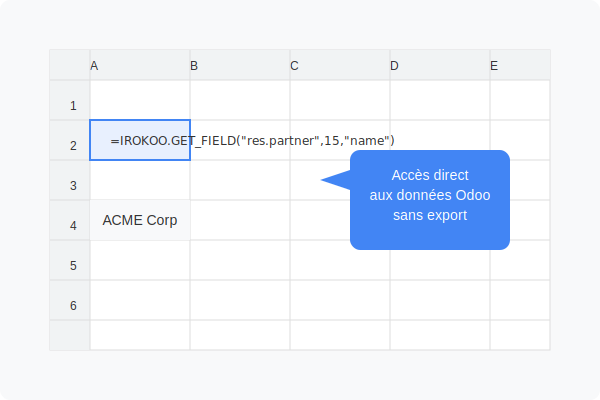
\includegraphics[width=0.6\textwidth]{feature1.png}
    \caption{Exemple d'utilisation des formules dans une feuille de calcul}
\end{figure}

\section{Liste des formules disponibles}

\subsection{IROKOO.GET\_FIELD}
\begin{tcolorbox}[title=Description]
Récupère la valeur d'un champ spécifique pour un enregistrement donné dans n'importe quel modèle Odoo.
\end{tcolorbox}

\subsubsection{Syntaxe}
\begin{lstlisting}
=IROKOO.GET_FIELD(model, id, field)
\end{lstlisting}

\subsubsection{Paramètres}
\begin{itemize}
    \item \textbf{model} (chaîne) : Nom technique du modèle (ex: "res.partner")
    \item \textbf{id} (nombre) : ID de l'enregistrement
    \item \textbf{field} (chaîne) : Nom technique du champ (ex: "name", "email", "phone")
\end{itemize}

\subsubsection{Retourne}
La valeur du champ demandé.

\subsubsection{Exemple}
\begin{lstlisting}
=IROKOO.GET_FIELD("res.partner", 1, "name")
\end{lstlisting}
Retourne le nom du partenaire ayant l'ID 1.

\subsubsection{Exemple avec champ relationnel}
\begin{lstlisting}
=IROKOO.GET_FIELD("sale.order", 123, "partner_id.name")
\end{lstlisting}
Retourne directement le nom du client associé à la commande de vente ayant l'ID 123, en accédant au champ \texttt{name} à travers la relation \texttt{partner\_id}.

\begin{tip}
Cette formule fonctionne avec tous les types de champs, y compris les champs relationnels. Pour les champs relationnels, le contenu retourné sera automatiquement formaté de manière appropriée.
\end{tip}

\subsection{IROKOO.GET\_IDS}
\begin{tcolorbox}[title=Description]
Récupère les IDs des enregistrements d'un modèle qui correspondent aux critères de filtre spécifiés.
\end{tcolorbox}

\subsubsection{Syntaxe}
\begin{lstlisting}
=IROKOO.GET_IDS(model, order, direction, limit, filters)
\end{lstlisting}

\subsubsection{Paramètres}
\begin{itemize}
    \item \textbf{model} (chaîne) : Nom technique du modèle (ex: "sale.order")
    \item \textbf{order} (chaîne) : Champ pour le tri (ex: "date\_order")
    \item \textbf{direction} (chaîne) : Direction du tri ("asc" ou "desc")
    \item \textbf{limit} (nombre) : Nombre maximum d'enregistrements à retourner (0 pour pas de limite)
    \item \textbf{filters} (chaîne) : Filtres séparés par des points-virgules
\end{itemize}

\subsubsection{Formats de filtre supportés}
\begin{itemize}
    \item \textbf{Format explicite} : \texttt{field:operator:value}
    \begin{itemize}
        \item Exemple : \texttt{state:in:draft,sent}
        \item Opérateurs : \texttt{=}, \texttt{!=}, \texttt{>}, \texttt{<}, \texttt{>=}, \texttt{<=}, \texttt{in}, \texttt{not in}, \texttt{ilike}, \texttt{like}
    \end{itemize}
    \item \textbf{Format simple} : \texttt{field=value}, \texttt{field>value}, etc.
    \begin{itemize}
        \item Exemple : \texttt{amount\_total>1000}
    \end{itemize}
    \item \textbf{Format recherche texte} : \texttt{field~value} pour recherches insensibles à la casse
    \begin{itemize}
        \item Exemple : \texttt{name~Comptabilité}
    \end{itemize}
    \item \textbf{Format avec \%} : \texttt{field=\%valeur\%} pour recherches partielles
    \begin{itemize}
        \item Exemple : \texttt{name=\%Dupont\%}
    \end{itemize}
\end{itemize}

\subsubsection{Retourne}
Une chaîne contenant les IDs séparés par des virgules.

\subsubsection{Exemple}
\begin{lstlisting}
=IROKOO.GET_IDS("sale.order", "date_order", "desc", 10, "state:in:draft,sent;date_order>2023-01-01")
\end{lstlisting}
Retourne les 10 derniers devis/commandes en état brouillon ou envoyé créés après le 1er janvier 2023.

\begin{warning}
Pour les filtres contenant des caractères spéciaux, assurez-vous d'utiliser le format explicite avec des deux-points comme séparateurs.
\end{warning}

\subsection{IROKOO.GET\_SUM}
\begin{tcolorbox}[title=Description]
Calcule la somme des valeurs d'un champ pour une liste d'IDs.
\end{tcolorbox}

\subsubsection{Syntaxe}
\begin{lstlisting}
=IROKOO.GET_SUM(model, field, ids)
\end{lstlisting}

\subsubsection{Paramètres}
\begin{itemize}
    \item \textbf{model} (chaîne) : Nom technique du modèle (ex: "sale.order")
    \item \textbf{field} (chaîne) : Nom technique du champ à sommer (ex: "amount\_untaxed")
    \item \textbf{ids} (chaîne) : Liste d'IDs séparés par des virgules (généralement le résultat de GET\_IDS)
\end{itemize}

\subsubsection{Retourne}
La somme des valeurs du champ pour les enregistrements spécifiés.

\subsubsection{Exemple}
\begin{lstlisting}
=IROKOO.GET_SUM("sale.order", "amount_untaxed", IROKOO.GET_IDS("sale.order", "date_order", "desc", 0, "state=sale"))
\end{lstlisting}
Calcule la somme des montants HT de toutes les commandes confirmées.

\begin{note}
Cette formule est particulièrement utile combinée avec GET\_IDS pour créer des rapports dynamiques.
\end{note}

\subsection{IROKOO.GET\_GROUPED\_IDS}
\begin{tcolorbox}[title=Description]
Regroupe les enregistrements selon un champ et calcule une valeur agrégée pour chaque groupe.
\end{tcolorbox}

\subsubsection{Syntaxe}
\begin{lstlisting}
=IROKOO.GET_GROUPED_IDS(model, group_by, aggregate_field, aggregate_function, filters, limit)
\end{lstlisting}

\subsubsection{Paramètres}
\begin{itemize}
    \item \textbf{model} (chaîne) : Nom technique du modèle
    \item \textbf{group\_by} (chaîne) : Champ utilisé pour le regroupement
    \item \textbf{aggregate\_field} (chaîne) : Champ à agréger
    \item \textbf{aggregate\_function} (chaîne) : Fonction d'agrégation : "sum", "avg", "count", "min", "max"
    \item \textbf{filters} (chaîne) : Filtres (même format que GET\_IDS)
    \item \textbf{limit} (nombre) : Nombre maximum de groupes à retourner
\end{itemize}

\subsubsection{Retourne}
Une chaîne contenant les valeurs du champ de regroupement, séparées par des virgules, pour les groupes classés par valeur agrégée décroissante.

\subsubsection{Exemple}
\begin{lstlisting}
=IROKOO.GET_GROUPED_IDS("sale.order", "partner_id", "amount_total", "sum", "state=sale", 5)
\end{lstlisting}
Retourne les IDs des 5 clients ayant généré le plus de chiffre d'affaires à travers les commandes confirmées.

\begin{tip}
Cette formule est idéale pour créer des analyses de type "Top N" ou pour identifier des tendances comme les clients les plus actifs, les produits les plus vendus, etc.
\end{tip}

\subsection{IROKOO.SUM\_BY\_DOMAIN}
\begin{tcolorbox}[title=Description]
Calcule directement la somme d'un champ pour les enregistrements correspondant à un domaine, sans nécessiter d'étape intermédiaire.
\end{tcolorbox}

\subsubsection{Syntaxe}
\begin{lstlisting}
=IROKOO.SUM_BY_DOMAIN(model, field, filters)
\end{lstlisting}

\subsubsection{Paramètres}
\begin{itemize}
    \item \textbf{model} (chaîne) : Nom technique du modèle
    \item \textbf{field} (chaîne) : Champ à sommer
    \item \textbf{filters} (chaîne) : Filtres (même format que GET\_IDS)
\end{itemize}

\subsubsection{Retourne}
La somme des valeurs du champ pour les enregistrements correspondant aux filtres.

\subsubsection{Exemple}
\begin{lstlisting}
=IROKOO.SUM_BY_DOMAIN("account.move.line", "balance", "account_id=401100;date>=2023-01-01;date<=2023-12-31")
\end{lstlisting}
Calcule le solde total des écritures comptables sur le compte fournisseurs 401100 pour l'année 2023.

\begin{figure}[H]
    \centering
    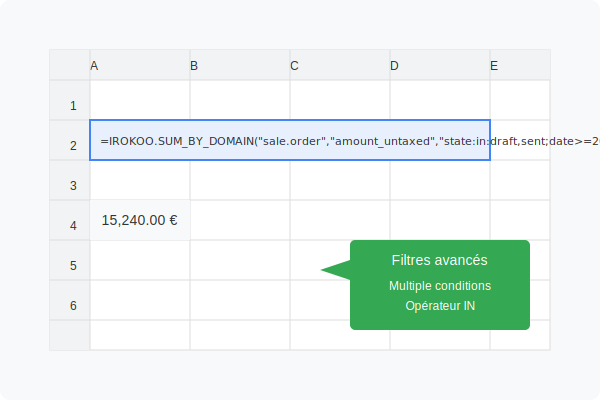
\includegraphics[width=0.8\textwidth]{feature2.png}
    \caption{Exemple d'utilisation de SUM\_BY\_DOMAIN avec filtres complexes}
\end{figure}

\subsection{IROKOO.COUNT\_BY\_DOMAIN}
\begin{tcolorbox}[title=Description]
Compte le nombre d'enregistrements correspondant à un domaine de filtrage, sans nécessiter d'étape intermédiaire.
\end{tcolorbox}

\subsubsection{Syntaxe}
\begin{lstlisting}
=IROKOO.COUNT_BY_DOMAIN(model, filters)
\end{lstlisting}

\subsubsection{Paramètres}
\begin{itemize}
    \item \textbf{model} (chaîne) : Nom technique du modèle
    \item \textbf{filters} (chaîne) : Filtres (même format que GET\_IDS)
\end{itemize}

\subsubsection{Retourne}
Le nombre d'enregistrements correspondant aux filtres.

\subsubsection{Exemple}
\begin{lstlisting}
=IROKOO.COUNT_BY_DOMAIN("sale.order", "state=sale;date_order>=2023-01-01;date_order<=2023-12-31")
\end{lstlisting}
Compte le nombre de commandes confirmées pour l'année 2023.

\begin{tip}
Utilisez cette formule à la place de \texttt{SUM\_BY\_DOMAIN} avec \texttt{"1"} comme champ pour obtenir un comptage plus précis et plus performant des enregistrements.
\end{tip}

\section{Utilisation avancée}

\subsection{Combinaison de formules}
Les formules peuvent être combinées pour créer des analyses complexes :
\begin{lstlisting}
=IROKOO.GET_SUM("sale.order", "amount_untaxed", 
  IROKOO.GET_IDS("sale.order", "date_order", "desc", 0, 
    "state=sale;partner_id=" & IROKOO.GET_GROUPED_IDS("sale.order", "partner_id", "amount_total", "sum", "state=sale", 1)
  )
)
\end{lstlisting}
Cette formule calcule le montant total des ventes pour le meilleur client.

\subsection{Filtres avec l'opérateur IN}
Utilisez l'opérateur IN pour filtrer sur plusieurs valeurs :
\begin{lstlisting}
=IROKOO.SUM_BY_DOMAIN("sale.order", "amount_total", "state:in:draft,sent,sale;date>=2023-01-01")
\end{lstlisting}

\subsection{Système de mise en cache}
Pour améliorer les performances, les formules implémentent désormais un système de mise en cache automatique :

\begin{itemize}
    \item Les résultats des requêtes sont stockés en mémoire pour une réutilisation rapide
    \item Le cache est automatiquement invalidé lors des changements de données
    \item Cette optimisation améliore considérablement la réactivité des tableaux de bord complexes
\end{itemize}

\begin{tip}
Grâce au système de cache, l'actualisation des données est beaucoup plus rapide lors de modifications mineures des filtres ou paramètres.
\end{tip}

\subsection{Conseils pour les performances}
\begin{itemize}
    \item Limiter le nombre d'appels de formules en utilisant SUM\_BY\_DOMAIN directement quand possible
    \item Utiliser des limites appropriées dans GET\_IDS pour réduire le volume de données
    \item Réutiliser les résultats de GET\_IDS dans plusieurs cellules plutôt que de répéter l'appel
    \item Préférer le format explicite field:operator:value pour les filtres complexes
\end{itemize}

\subsection{Utilisation de cellules de référence comme filtres}

Il est important de noter que les formules IROKOO.* ne sont pas directement compatibles avec les filtres globaux natifs d'Odoo Spreadsheet. Cependant, vous pouvez créer un système de filtrage efficace en utilisant des cellules de référence :

\begin{itemize}
    \item \textbf{Pour l'année} : Créez une cellule avec validation de données (liste déroulante) contenant les années disponibles, et référencez cette cellule dans vos formules
    \item \textbf{Pour la période} : Utilisez des cellules pour définir les dates de début et de fin, qui serviront de paramètres à toutes vos formules
    \item \textbf{Pour d'autres filtres} : Créez des cellules contenant les IDs des équipes, produits, etc., que vous souhaitez filtrer
\end{itemize}

Exemple de mise en place :
\begin{lstlisting}
D1: "Filtre par équipe"
D2: [liste déroulante avec IDs des équipes]
\end{lstlisting}

Puis dans vos formules, référencez cette cellule :
\begin{lstlisting}
=IROKOO.SUM_BY_DOMAIN("sale.order", "amount_untaxed", "state=sale;team_id=" & D2 & ";date_order>=" & TEXT(B2,"yyyy-mm-dd"))
\end{lstlisting}

Cette approche permet de mettre à jour dynamiquement toutes vos formules lorsque l'utilisateur change la valeur d'une cellule de filtrage.

\subsection{Gestion des dates}

Les formules ont été optimisées pour une meilleure gestion des filtres de date :

\begin{itemize}
    \item Les dates sont correctement formatées quel que soit le format de la cellule source
    \item Les formules attendent patiemment le chargement complet des données avant d'afficher les résultats
    \item Les textes de chargement sont localisés en français ("Chargement des données en cours...")
\end{itemize}

Pour une utilisation optimale avec des filtres de date :

\begin{lstlisting}
=IROKOO.SUM_BY_DOMAIN("sale.order", "amount_total", "date_order>=" & TEXT(B2,"yyyy-mm-dd") & ";date_order<=" & TEXT(B3,"yyyy-mm-dd"))
\end{lstlisting}

\subsection{Conseils pour l'optimisation}

\begin{itemize}
    \item Utilisez des cellules de référence pour les paramètres communs (dates, filtres)
    \item Minimisez le nombre d'appels à IROKOO.GET\_IDS en stockant les résultats dans des cellules intermédiaires
    \item Privilégiez IROKOO.SUM\_BY\_DOMAIN pour les calculs directs plutôt que des formules imbriquées complexes
    \item Pour les tableaux très volumineux, segmentez vos requêtes par période pour améliorer les performances
\end{itemize}

Ce tableau de bord vous donne un point de départ pour créer vos propres analyses adaptées à vos besoins spécifiques. Les formules peuvent être modifiées et combinées pour répondre à différentes questions métier.

\section{Dépannage}

\subsection{Erreurs courantes}
\begin{itemize}
    \item \textbf{"Tous les paramètres sont requis"} : Vérifiez que tous les arguments obligatoires sont fournis
    \item \textbf{"Chargement des données en cours..."} : Patientez, les données sont en cours de chargement
    \item \textbf{"Aucun résultat trouvé"} : Les filtres ne correspondent à aucun enregistrement
    \item \textbf{"Erreur lors de l'exécution de la recherche"} : Vérifiez la syntaxe des filtres et l'existence du modèle
\end{itemize}

\subsection{Problèmes de chargement}
Si vous rencontrez des problèmes avec les formules affichant "Chargement des données en cours..." trop longtemps :
\begin{itemize}
    \item Vérifiez que les filtres de date sont correctement formatés avec \texttt{TEXT(date,"yyyy-mm-dd")}
    \item Réduisez la plage de données en ajoutant des filtres plus restrictifs
    \item Vérifiez les performances de votre serveur Odoo, des requêtes complexes peuvent prendre du temps
    \item Consultez les logs du navigateur pour identifier d'éventuelles erreurs JavaScript
\end{itemize}

\subsection{Problèmes d'accès}
\begin{itemize}
    \item Les formules respectent les droits d'accès de l'utilisateur
    \item Un utilisateur ne peut accéder qu'aux données auxquelles il a droit
    \item Si une formule retourne une erreur pour certains utilisateurs, vérifiez leurs droits d'accès
\end{itemize}

\begin{warning}
Si vous rencontrez des problèmes d'accès, assurez-vous que l'utilisateur a les droits nécessaires pour accéder au modèle et aux champs spécifiés dans la formule.
\end{warning}

\section{Aspects techniques et défis rencontrés}

Au cours du développement de ce module, nous avons dû faire face à plusieurs défis techniques. Cette section présente les principales difficultés rencontrées et les solutions mises en œuvre pour les surmonter. Ces informations peuvent être utiles pour les développeurs souhaitant étendre les fonctionnalités ou comprendre les choix d'implémentation.

\subsection{Chargement asynchrone des données}

\begin{itemize}
    \item \textbf{Problème} : Les formules s'exécutent de manière asynchrone, ce qui peut entraîner des affichages "Chargement des données en cours..." persistants, notamment avec les filtres de date.
    \item \textbf{Solution} : Implémentation d'un système de gestion avancé des promesses JavaScript, avec détection de l'état de chargement et retry automatique en cas d'échec.
    \item \textbf{Résultat} : Une expérience utilisateur plus fluide et des formules qui attendent correctement que les données soient disponibles.
\end{itemize}

\subsection{Simulation de GET\_FIELD pour résoudre les blocages}

\begin{itemize}
    \item \textbf{Problème} : Dans certaines situations complexes impliquant des champs relationnels et des filtres de date, les formules GET\_GROUPED\_IDS restaient bloquées en chargement.
    \item \textbf{Solution} : Nous avons implémenté une technique de "simulation" de GET\_FIELD dans le code de GET\_GROUPED\_IDS, permettant de pré-charger les données relationnelles nécessaires avant de commencer le calcul d'agrégation.
    \item \textbf{Exemple} : Pour les filtres comme "order\_id.date\_order>=", le module pré-charge maintenant les dates avant de filtrer, évitant ainsi les blocages.
\end{itemize}

\subsection{Système de cache intelligent}

\begin{itemize}
    \item \textbf{Problème} : Répétition de requêtes identiques, particulièrement sur les tableaux de bord complexes, entraînant des performances insuffisantes.
    \item \textbf{Solution} : Implémentation d'un système de cache à deux niveaux :
    \begin{itemize}
        \item Cache de premier niveau pour les résultats de recherche (domaines)
        \item Cache de second niveau pour les résultats d'agrégation (sommes, comptes, etc.)
    \end{itemize}
    \item \textbf{Avantage} : Réduction drastique du nombre de requêtes, avec invalidation automatique du cache lors des modifications de données.
\end{itemize}

\subsection{Gestion des erreurs et résilience}

\begin{itemize}
    \item \textbf{Problème} : Certaines formules échouaient silencieusement ou bloquaient l'interface utilisateur lors d'erreurs.
    \item \textbf{Solutions} : 
    \begin{itemize}
        \item Localisation française des messages d'erreur pour une meilleure compréhension
        \item Implémentation d'un système de logging détaillé dans la console navigateur
        \item Mécanisme de fallback permettant de retourner des résultats partiels plutôt qu'une erreur complète
    \end{itemize}
    \item \textbf{Résultat} : Un module plus robuste qui guide l'utilisateur en cas de problème.
\end{itemize}

\subsection{Optimisation de COUNT\_BY\_DOMAIN}

\begin{itemize}
    \item \textbf{Problème} : Utilisation inefficace de SUM\_BY\_DOMAIN avec "1" comme champ pour compter les enregistrements.
    \item \textbf{Solution} : Création d'une formule dédiée COUNT\_BY\_DOMAIN utilisant l'API native de comptage d'Odoo.
    \item \textbf{Bénéfice} : Performances améliorées et meilleure lisibilité des formules dans les tableaux de bord.
\end{itemize}

\subsection{Conseils de développement pour l'extension}

Pour les développeurs souhaitant étendre ce module avec de nouvelles formules, nous recommandons de :

\begin{itemize}
    \item Suivre le pattern de gestion asynchrone mis en place pour assurer la compatibilité
    \item Intégrer vos formules dans le système de cache existant
    \item Tester intensivement avec des cas complexes impliquant des champs relationnels et des filtres de date
    \item Utiliser la console du navigateur pour déboguer lors du développement (les logs détaillés y sont disponibles)
    \item Prévoir des mécanismes de fallback pour retourner des résultats partiels plutôt que des erreurs complètes
\end{itemize}

\begin{tip}
Pour le développement de nouvelles formules, inspectez le code source de GET\_GROUPED\_IDS qui illustre les meilleures pratiques de gestion asynchrone des données et d'utilisation du cache.
\end{tip}

\section{Exemple de tableau de bord}

Cette section présente un exemple complet de construction d'un tableau de bord d'analyse des ventes à l'aide des formules du module Spreadsheet Evolution.

\subsection{Objectif du tableau de bord}

Notre tableau de bord vise à répondre aux questions suivantes :
\begin{itemize}
    \item Quelle est l'évolution mensuelle des ventes sur l'année en cours ?
    \item Qui sont nos 5 meilleurs clients et leur chiffre d'affaires ?
    \item Quels sont nos 5 produits les plus vendus (en valeur et en quantité) ?
    \item Quel est le taux de conversion de nos devis en commandes ?
    \item Comment se répartissent nos ventes par équipe de vente ?
\end{itemize}

\subsection{Architecture à deux feuilles}

Une bonne pratique pour construire des tableaux de bord complexes consiste à utiliser deux feuilles distinctes :

\begin{itemize}
    \item \textbf{Feuille principale} : "Tableau de bord Ventes" - Contient la présentation et les visualisations
    \item \textbf{Feuille de données} : "Data" - Stocke les requêtes complexes et les résultats intermédiaires
\end{itemize}

Cette architecture présente plusieurs avantages :
\begin{itemize}
    \item Les requêtes complexes (notamment GET\_GROUPED\_IDS) sont isolées et plus faciles à déboguer
    \item Les formules de la feuille principale restent plus lisibles et maintenues
    \item Le cache fonctionne mieux car les requêtes similaires sont centralisées
    \item L'affichage est plus propre, la feuille de données pouvant être masquée
\end{itemize}

\subsection{Implémentation étape par étape}

\subsubsection{Étape 1 : Création et paramétrage des feuilles}

\begin{itemize}
    \item Créez une première feuille nommée "Tableau de bord Ventes"
    \item Créez une seconde feuille nommée "Data"
    \item Dans les paramètres de la feuille "Data", vous pouvez masquer les colonnes contenant les formules complexes
\end{itemize}

\subsubsection{Étape 2 : Préparation des données de référence dans l'onglet principal}

Dans la feuille principale, configurez les filtres globaux :

\begin{lstlisting}
C1: "Année en cours"
D1: =YEAR(TODAY())
C2: "Date début"
D2: =DATE(D1,1,1)
C3: "Date fin"
D3: =DATE(D1,12,31)
\end{lstlisting}

\subsubsection{Étape 3 : Préparation des requêtes complexes dans la feuille Data}

Dans la feuille "Data", préparez les requêtes de regroupement qui seront utilisées à plusieurs endroits :

\begin{lstlisting}
# Top 5 clients par montant de vente
B2: =IROKOO.GET_GROUPED_IDS("sale.order", "partner_id", "amount_total", "sum", "state=sale;date_order>=" & TEXT('Tableau de bord Ventes'!D2,"yyyy-mm-dd") & ";date_order<=" & TEXT('Tableau de bord Ventes'!D3,"yyyy-mm-dd"), 5)

# Top 5 produits par montant de vente
B6: =IROKOO.GET_GROUPED_IDS("sale.order.line", "product_id", "price_subtotal", "sum", "order_id.state=sale;order_id.date_order>=" & TEXT('Tableau de bord Ventes'!D2,"yyyy-mm-dd") & ";order_id.date_order<=" & TEXT('Tableau de bord Ventes'!D3,"yyyy-mm-dd"), 5)

# Top équipes de vente
B8: =IROKOO.GET_GROUPED_IDS("sale.order", "team_id", "amount_total", "sum", "state=sale;date_order>=" & TEXT('Tableau de bord Ventes'!D2,"yyyy-mm-dd") & ";date_order<=" & TEXT('Tableau de bord Ventes'!D3,"yyyy-mm-dd"), 2)
\end{lstlisting}

\begin{warning}
Il est crucial de préparer l'onglet "Data" avant de configurer les formules dans l'onglet principal. Sinon, vous obtiendrez des erreurs de référence puisque les formules de l'onglet principal feront référence à des données qui n'existent pas encore.
\end{warning}

\begin{tip}
Ajoutez des commentaires explicatifs dans la feuille Data à côté des formules pour identifier facilement leur fonction. Ces commentaires peuvent être mis dans la colonne A.
\end{tip}

\subsubsection{Étape 4 : Configuration des colonnes de dates et périodes}

Retournez dans l'onglet principal et configurez les périodes mensuelles :

\begin{lstlisting}
# Colonnes pour les dates (peuvent être cachées)
A6: =MONTH.START(B6)           # Début du mois
B6: =EOMONTH(D2,0)             # Fin du premier mois
A7: =MONTH.START(B7)           # Début du mois suivant
B7: =EOMONTH(B6,1)             # Fin du mois suivant
# Etc. pour chaque mois...
\end{lstlisting}

\subsubsection{Étape 5 : Évolution mensuelle des ventes}

Configurez maintenant l'affichage des données mensuelles :

\begin{lstlisting}
# Noms des mois et données
C5: "Mois"
D5: "Total ventes HT"
E5: "Nbre cmde"

C6: "Janvier"
D6: =IROKOO.SUM_BY_DOMAIN("sale.order", "amount_untaxed", "state=sale;date_order>=" & TEXT(A6,"yyyy-mm-dd") & ";date_order<=" & TEXT(B6,"yyyy-mm-dd"))
E6: =IROKOO.COUNT_BY_DOMAIN("sale.order", "state=sale;date_order>=" & TEXT(A6,"yyyy-mm-dd") & ";date_order<=" & TEXT(B6,"yyyy-mm-dd"))

# Répéter pour tous les mois...

# Ajouter un total pour le semestre
C18: "TOTAL S1"
D18: =SUM(D6:D11)
E18: =SUM(E6:E11)
\end{lstlisting}

\subsubsection{Étape 6 : Configuration des Top 5 clients}

Utilisez maintenant les données regroupées de la feuille "Data" pour afficher les meilleurs clients :

\begin{lstlisting}
H4: "Top 5 clients"
H5: "Nom"
I5: "Montant cde"

# Colonne pour stocker les IDs (peut être cachée)
G5: "ID"
G6: =TRANSPOSE(INDEX(SPLIT(Data!B2,","),1))

# Affichage du nom et montant pour chaque client
H6: =IFERROR(IROKOO.GET_FIELD("res.partner",G6,"name"),"")
I6: =IFERROR(IROKOO.SUM_BY_DOMAIN("sale.order", "amount_untaxed", "state=sale;partner_id=" & G6 & ";date_order>=" & TEXT(D$2,"yyyy-mm-dd") & ";date_order<=" & TEXT(D$3,"yyyy-mm-dd")),"")

# Répéter pour les lignes suivantes (G7-I10) en incrémentant les références
\end{lstlisting}

\subsubsection{Étape 7 : Configuration des Top 5 produits}

Même principe pour les produits, en utilisant le regroupement stocké dans la feuille "Data" :

\begin{lstlisting}
K4: "Top 5 produits"
K5: "Produit"
L5: "Qté"
M5: "Montant cde"

# Colonne pour stocker les IDs (peut être cachée)
J5: "ID"
J6: =TRANSPOSE(INDEX(SPLIT(Data!B6,","),1))

# Affichage des informations pour chaque produit
K6: =IROKOO.GET_FIELD("product.product",J6,"name")
L6: =IROKOO.SUM_BY_DOMAIN("sale.order.line", "product_uom_qty", "order_id.state=sale;product_id=" & J6 & ";order_id.date_order>=" & TEXT(D2,"yyyy-mm-dd") & ";order_id.date_order<=" & TEXT(D3,"yyyy-mm-dd"))
M6: =IROKOO.SUM_BY_DOMAIN("sale.order.line", "price_subtotal", "order_id.state=sale;product_id=" & J6 & ";order_id.date_order>=" & TEXT(D2,"yyyy-mm-dd") & ";order_id.date_order<=" & TEXT(D3,"yyyy-mm-dd"))

# Répéter pour les lignes suivantes
\end{lstlisting}

\subsubsection{Étape 8 : Taux de conversion des devis}

Calculons le taux de conversion des devis en commandes :

\begin{lstlisting}
C24: "Taux de conversion des devis"
A25: "Nombre total de devis"
D25: =IROKOO.COUNT_BY_DOMAIN("sale.order", "date_order>=" & TEXT(D2,"yyyy-mm-dd") & ";date_order<=" & TEXT(D3,"yyyy-mm-dd"))
A26: "Nombre de commandes confirmées"
D26: =IROKOO.COUNT_BY_DOMAIN("sale.order", "state=sale;date_order>=" & TEXT(D2,"yyyy-mm-dd") & ";date_order<=" & TEXT(D3,"yyyy-mm-dd"))
A27: "Taux de conversion"
D27: =IF(D25=0,0,D26/D25)
\end{lstlisting}

\subsubsection{Étape 9 : Répartition par équipe de vente}

Analysons les performances par équipe de vente en utilisant la requête stockée dans la feuille "Data" :

\begin{lstlisting}
# Colonne cachée pour les IDs d'équipe
G24: "ID"
G25: =TRANSPOSE(INDEX(SPLIT(Data!B8,","),1))

H24: "Répartition par équipe de vente"
H25: =IROKOO.GET_FIELD("crm.team",G25,"name")
I25: =IROKOO.SUM_BY_DOMAIN("sale.order", "amount_untaxed", "state=sale;team_id=" & G25 & ";date_order>=" & TEXT(D2,"yyyy-mm-dd") & ";date_order<=" & TEXT(D3,"yyyy-mm-dd"))
\end{lstlisting}

\subsubsection{Étape 10 : Ajout de graphiques}

Pour finaliser le tableau de bord, ajoutez deux graphiques principaux :

\begin{itemize}
    \item Un graphique en barres montrant l'évolution mensuelle des ventes (utilisant la plage D6:D17 pour les données et C6:C17 pour les étiquettes)
    \item Un graphique en secteurs montrant la répartition par clients (utilisant la plage I6:I17 pour les données et H6:H17 pour les étiquettes)
\end{itemize}

\subsection{Astuces pour optimiser le tableau de bord}

\begin{itemize}
    \item \textbf{Masquer les colonnes techniques} : Les colonnes contenant uniquement des IDs ou des calculs intermédiaires peuvent être masquées pour améliorer la lisibilité
    \item \textbf{Utiliser IFERROR} : Cette fonction permet de gérer élégamment les cas où des données seraient absentes
    \item \textbf{Centraliser les requêtes complexes} : Placer les formules GET\_GROUPED\_IDS dans la feuille "Data" améliore les performances et facilite la maintenance
    \item \textbf{Référencer la feuille principale pour les filtres} : Utiliser 'Tableau de bord Ventes'!D2 comme référence garantit que toutes les requêtes utilisent les mêmes paramètres
    \item \textbf{Utiliser les fonctions TRANSPOSE et INDEX avec SPLIT} : Cette combinaison permet d'extraire facilement les IDs individuels de résultats de regroupement
\end{itemize}

\begin{tip}
Pour extraire un élément spécifique d'un résultat de type liste (comme celui retourné par GET\_GROUPED\_IDS), utilisez la combinaison TRANSPOSE(INDEX(SPLIT(résultat,","),index\_voulu)) où index\_voulu est le numéro de l'élément à extraire (1 pour le premier).
\end{tip}

Ce tableau de bord vous donne un point de départ solide pour créer vos propres analyses adaptées à vos besoins spécifiques. Les techniques utilisées ici peuvent être facilement adaptées pour suivre d'autres indicateurs clés ou pour créer des tableaux de bord pour d'autres modules d'Odoo.

\end{document} 